\documentclass[conference]{IEEEtran}
\IEEEoverridecommandlockouts
\usepackage{cite}
\usepackage{amsmath,amssymb,amsfonts}
\usepackage{algorithmic}
\usepackage{graphicx}
\usepackage{textcomp}
\usepackage{xcolor}
\usepackage{booktabs}
\usepackage{array}
\usepackage{tabularx}
\usepackage{hyperref}
\usepackage{tikz}
\usetikzlibrary{shapes.geometric,arrows.meta,positioning,backgrounds,fit}
\definecolor{stagegreen}{RGB}{209,243,209}
\definecolor{stageblue}{RGB}{210,228,255}
\definecolor{stagegray}{RGB}{235,235,235}
\definecolor{stagered}{RGB}{255,210,210}
\newcommand{\ghfile}[2]{\href{https://github.com/rah-ds/Wikipedia_Dispute_Models/blob/main/#1}{\texttt{#2}}}
\newcommand{\ghrepo}{\url{https://github.com/rah-ds/Wikipedia_Dispute_Models}}
\def\BibTeX{{\rm B\kern-.05em{\sc i\kern-.025em b}\kern-.08em
    T\kern-.1667em\lower.7ex\hbox{E}\kern-.125emX}}
\begin{document}

\title{From Revert to Remedy:\\Process Modeling Wikipedia's Dispute Escalation%
\thanks{This work was completed as part of the UVA MSDS DS~6015 Capstone
  in collaboration with Lexipedia and the Wikimedia Foundation.
  Code: \protect\ghrepo}
}

\author{
\IEEEauthorblockN{Louis Cocks}
\IEEEauthorblockA{\textit{School of Data Science} \\
\textit{University of Virginia}\\
Charlottesville, VA, USA \\
lcocks@virginia.edu}
\and
\IEEEauthorblockN{Katherine Kelleher}
\IEEEauthorblockA{\textit{School of Data Science} \\
\textit{University of Virginia}\\
Charlottesville, VA, USA}
\and
\IEEEauthorblockN{Ryan Healy}
\IEEEauthorblockA{\textit{School of Data Science} \\
\textit{University of Virginia}\\
Charlottesville, VA, USA \\
rah5ff@virginia.edu}
}

\maketitle

\begin{abstract}
Wikipedia operates as a self-governing encyclopedia in which volunteer editors
resolve conflict through a five-stage escalation pathway, from talk page
discussion to binding arbitration. We formalize this pathway as a Business
Process Model and Notation (BPMN~2.0) swimlane model, mapping participants,
gateways, and remedial outcomes across all five intervention venues. The model
is grounded in a structured dataset of approximately 170 Arbitration Committee
(ArbCom) cases spanning 2004--2023, collected via a purpose-built pipeline
against the MediaWiki, ORES, Pageviews, and XTools APIs. An interactive
dashboard renders each case as a navigable BPMN diagram alongside analytics
covering case duration, statement distributions, party types, and remedy
verbs. Across five high-profile sample cases, we find that bilateral edit-war
pairs drive the majority of reverts, that over 60\% of ArbCom participants
are traceable to earlier ANI threads, and that abuse-filter hit counts reliably
distinguish sanctioned from unsanctioned editors. The process model and dataset
are released publicly to support reproducible research on collaborative online
governance.
\end{abstract}

\begin{IEEEkeywords}
Wikipedia, BPMN, process modeling, dispute resolution, arbitration, edit wars,
collaborative governance, escalation prediction, MediaWiki API
\end{IEEEkeywords}

% -----------------------------------------------------------------------
\section{Introduction}
% -----------------------------------------------------------------------

Every hour, editors on the English Wikipedia open thousands of disputes. Most
die quietly on article talk pages. A few harden into edit wars, climb through
noticeboards, and end in binding sanctions from the Arbitration Committee
(ArbCom), Wikipedia's court of last resort. Despite decades of study, no
prior work has given this escalation a formal process model, leaving
practitioners and researchers without a shared, executable representation of
how conflict moves through the system.

We address this gap with three contributions: (1)~a BPMN~2.0 swimlane model
of the complete dispute escalation pathway; (2)~a structured dataset of
$\sim$170 ArbCom cases that grounds the model in 20 years of real cases; and
(3)~an interactive dashboard~\cite{b_dashboard} that renders each case as a
navigable BPMN diagram alongside analytics covering duration, parties, and
remedies. The process model makes implicit governance logic explicit: gateways
represent policy decisions, swimlane boundaries mark jurisdictional
transitions, and timer events capture escalation deadlines.

% -----------------------------------------------------------------------
\section{Background}
% -----------------------------------------------------------------------

\subsection{Wikipedia's Governance Structure}

Wikipedia's English edition is self-governed by a layered hierarchy:
\emph{editors} (any contributor), \emph{administrators} (elected, can block
and protect), \emph{bureaucrats} (grant admin rights), and the
\emph{Arbitration Committee} (ArbCom), an annually elected body that
issues binding conduct sanctions~\cite{b_wikistats}. Three core content
policies (Neutral Point of View, Verifiability, and No Original
Research) define the terrain of most disputes.

\subsection{The Five-Stage Escalation Pathway}

Wikipedia employs \emph{graduated intervention}: binding force increases as
lower-level mechanisms fail~\cite{b_wp_lifecycle}. Fig.~\ref{fig:bpmn} shows
our BPMN swimlane model of this pathway, with lanes separating the four
participant tiers and XOR gateways encoding the ``resolved vs.~escalate''
policy decision at each stage.

% ── BPMN-style swimlane figure ────────────────────────────────────────
\begin{figure*}[tb]
\centering
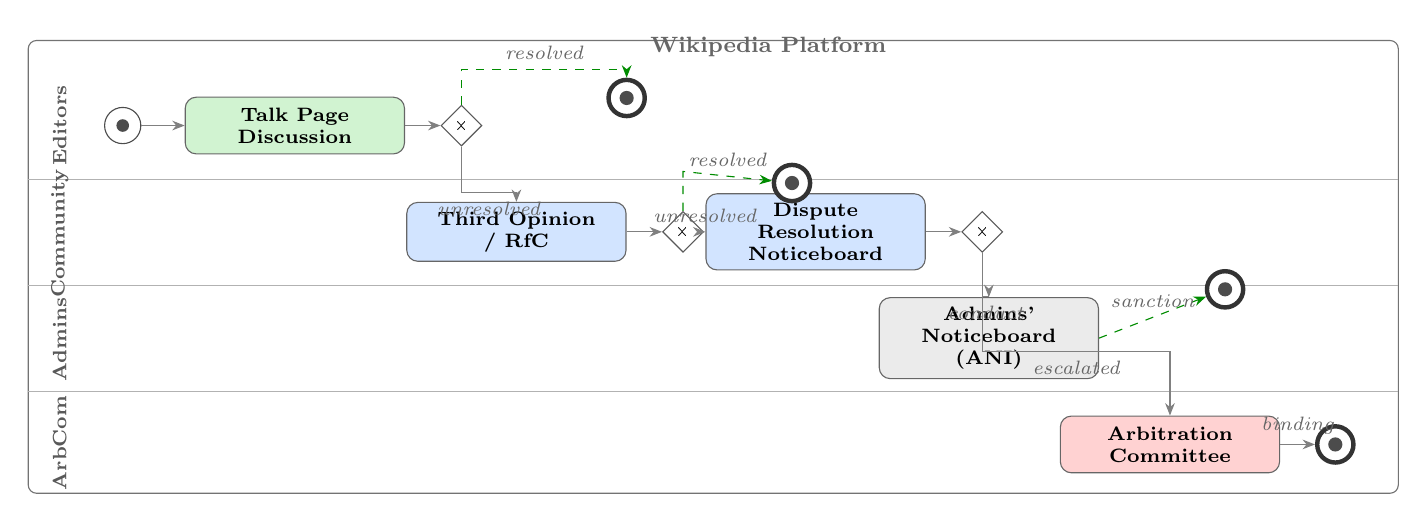
\begin{tikzpicture}[
  %% styles
  task/.style={rectangle, rounded corners=4pt,
               draw=black!60, fill=#1,
               text width=2.55cm, minimum height=0.72cm,
               align=center, font=\scriptsize\bfseries},
  gw/.style={diamond, draw=black!65, fill=white,
             inner sep=0pt, minimum size=0.52cm,
             font=\tiny, aspect=1},
  ev/.style={circle, draw=black!70, fill=white,
             minimum size=0.46cm, inner sep=0pt},
  evend/.style={circle, draw=black!80, fill=white, line width=1.6pt,
                minimum size=0.46cm, inner sep=0pt},
  arr/.style={-{Stealth[length=4.5pt,width=3.5pt]}, draw=black!50, thin},
  reslv/.style={arr, dashed, draw=green!55!black},
  lbl/.style={font=\scriptsize\itshape, text=black!60},
  lanelbl/.style={font=\scriptsize\bfseries, rotate=90, anchor=center,
                  text=black!65},
]

%%
%% Lane heights (y-centres)
%%
\def\Ly{0}      % Lane 4 : ArbCom
\def\Lya{1.35}  % Lane 3 : Admins
\def\Lyb{2.70}  % Lane 2 : Community
\def\Lyc{4.05}  % Lane 1 : Editors

%% ------ pool border + lane dividers -----------------------------------
\def\poolW{16.6}  \def\poolH{5.15}  \def\laneX{-0.7}
\draw[draw=black!55, rounded corners=3pt]
  (\laneX,-0.62) rectangle (\poolW+0.1, \poolH-0.02);
\draw[black!30] (\laneX,0.67) -- (\poolW+0.1,0.67);
\draw[black!30] (\laneX,2.02) -- (\poolW+0.1,2.02);
\draw[black!30] (\laneX,3.37) -- (\poolW+0.1,3.37);

%% lane labels (vertical, centred in each band)
\node[lanelbl] at (-0.3, \Lyc+0.0) {Editors};
\node[lanelbl] at (-0.3, \Lyb-0.02) {Community};
\node[lanelbl] at (-0.3, \Lya-0.02) {Admins};
\node[lanelbl] at (-0.3, \Ly+0.02)  {ArbCom};

%% pool label
\node[font=\footnotesize\bfseries, text=black!60, anchor=north]
  at (\poolW/2+0.4, \poolH+0.15) {\textsc{Wikipedia Platform}};

%% ------ elements -------------------------------------------------------

%% Start
\node[ev] (start) at (0.5, \Lyc) {};
\fill[black!70] (start.center) circle (0.08cm);

%% Talk Page (Editors lane)
\node[task=stagegreen, right=0.55cm of start] (talk)
  {Talk Page\\Discussion};

%% GW1: resolved?
\node[gw, right=0.45cm of talk] (gw1) {\texttimes};

%% 3O/RfC (Community lane)
\node[task=stageblue] (rfc) at (5.5, \Lyb)
  {Third Opinion\\/ RfC};

%% GW2: resolved?
\node[gw, right=0.45cm of rfc] (gw2) {\texttimes};

%% DRN (Community lane)
\node[task=stageblue] (drn) at (9.3, \Lyb)
  {Dispute Resolution\\Noticeboard};

%% GW3: resolved / conduct?
\node[gw, right=0.45cm of drn] (gw3) {\texttimes};

%% ANI (Admins lane)
\node[task=stagegray] (ani) at (11.5, \Lya)
  {Admins'\\Noticeboard (ANI)};

%% ArbCom (ArbCom lane)
\node[task=stagered] (arb) at (13.8, \Ly)
  {Arbitration\\Committee};

%% End events
\node[evend] (eok1) at (6.9, \Lyc+0.35)  {}; \fill[black!70] (eok1.center) circle (0.09cm);
\node[evend] (eok2) at (9.0, \Lyb+0.62)  {}; \fill[black!70] (eok2.center) circle (0.09cm);
\node[evend] (eok3) at (14.5,\Lya+0.62)  {}; \fill[black!70] (eok3.center) circle (0.09cm);
\node[evend] (efin) at (15.9, \Ly)       {}; \fill[black!70] (efin.center) circle (0.09cm);

%% ------ sequence flows ------------------------------------------------
\draw[arr] (start) -- (talk);
\draw[arr] (talk)  -- (gw1);

%% gw1 down → rfc
\draw[arr] (gw1.south) -- ++(0,-0.58)
    -| node[near start, below, lbl]{unresolved} (rfc);
%% gw1 right → resolved end
\draw[reslv] (gw1.north) -- ++(0,0.45)
    -| node[near start, above, lbl]{resolved} (eok1);

\draw[arr] (rfc) -- (gw2);
%% gw2 right → drn
\draw[arr] (gw2.east) -- node[above, lbl]{unresolved} (drn);
%% gw2 up → resolved end
\draw[reslv] (gw2.north) -- ++(0,0.50)
    -- node[above, lbl]{resolved} (eok2);

\draw[arr] (drn) -- (gw3);
%% gw3 south → ani
\draw[arr] (gw3.south) -- ++(0,-0.55)
    -| node[near start, below, lbl]{conduct} (ani);
%% gw3 south-south → arb
\draw[arr] (gw3.south) -- ++(0,-0.55) -- ++(0,-0.70)
    -| node[near start, below, lbl]{escalated} (arb);
%% ani → resolved
\draw[reslv] (ani.east) -- node[above, lbl]{sanction} (eok3);
%% arb → end
\draw[arr] (arb) -- node[above, lbl]{binding} (efin);

\end{tikzpicture}
\caption{BPMN~2.0 swimlane model of Wikipedia's dispute escalation.
  Lanes separate participant tiers; \texttimes-gateways encode the
  ``resolved vs.~escalate'' policy decision at each stage.
  Dashed green flows indicate resolved exits; solid flows indicate
  escalation. Start and end events follow BPMN~2.0 notation.}
\label{fig:bpmn}
\end{figure*}
% ── end figure ────────────────────────────────────────────────────────

\noindent\textbf{Stage~1: Talk Page.} Editors must attempt resolution
directly on the article talk page before escalating. The DRN requires evidence
of discussion spanning at least two days~\cite{b_wp_drn}.

\noindent\textbf{Stage~2: Third Opinion / RfC.} A Third Opinion involves
exactly two disputants and a volunteer referee. Requests for Comment (RfC)
bring in broader community input for multi-party or policy disputes.

\noindent\textbf{Stage~3: Dispute Resolution Noticeboard (DRN).}
Volunteer moderators facilitate \emph{content} disputes only. Cases close as
consensus, referral, or unresolved~\cite{b_wp_drn}.

\noindent\textbf{Stage~4: Administrators' Noticeboard Incidents (ANI).}
\emph{Conduct} violations (harassment, sock-puppetry, edit warring) enter the
admin tier here. Administrators may sanction without formal proceedings.

\noindent\textbf{Stage~5: Arbitration Committee (ArbCom).}
The court of last resort for conduct. Cases span five structured subpages
(main, evidence, workshop, proposed decision, remedies). Decisions are
binding: site bans, topic restrictions, supervised editing.

\subsection{BPMN as a Formalism for Online Governance}

Business Process Model and Notation~2.0 (BPMN) is an ISO/IEC standard
graphical language for specifying workflows~\cite{b_bpmn}. Its constructs
map naturally onto Wikipedia's governance: \emph{tasks} correspond to
discussion and decision activities; \emph{swimlanes} encode jurisdictional
boundaries (editors, community volunteers, administrators, committee);
\emph{XOR gateways} represent binary policy decisions (``resolved?'');
and \emph{end events} distinguish voluntary resolution from imposed remedy.
Formalizing the process this way exposes structures (gateway fan-out,
inter-lane message flows, timer boundary events for escalation
deadlines) that informal narrative descriptions obscure.

% -----------------------------------------------------------------------
\section{Related Work}
% -----------------------------------------------------------------------

\subsection{Process Mining and Online Governance}

Process mining extracts process models from event logs~\cite{b_vander2012}.
Applied to Wikipedia, revision histories constitute precisely such logs:
each revision is a timestamped event with actor, artifact, and action. Prior
work has not applied formal process mining tools to the dispute resolution
pathway; we take a step in this direction by constructing BPMN models from
case subpages and validating them against collected event logs.

\subsection{Edit War Detection}

Kittur et al.~\cite{b_kittur2007} introduced foundational metrics for detecting
conflict through revert patterns, showing that mutual reversion sequences
reliably identify edit wars. In subsequent work, Kittur and
Kraut~\cite{b_kittur2010} extended this analysis to coordination breakdowns in
online production groups more broadly. Yasseri et al.~\cite{b_yasseri2012}
quantified edit wars globally using a \emph{mutually reverting edit index}
(M-index), finding that politically, religiously, and geographically
contentious topics consistently attract the most conflict.

\subsection{Dispute Resolution Mechanisms}

Wikipedia's own documentation describes a graduated series of venues through
which disputes are expected to travel~\cite{b_wp_disputes}.
Geiger and Ribes~\cite{b_geiger2010} examined Wikipedia's anti-vandalism
infrastructure through an ethnographic lens, documenting how bots and human
editors collaborate in governance. Taraborelli and Ciampaglia~\cite{b_taraborelli2010}
analyzed Articles for Deletion (AfD) as a governance mechanism, providing a
model for studying how consensus forms under conflict. Halfaker et
al.~\cite{b_halfaker2013} documented the hardening of Wikipedia's newcomer
environment, connecting dispute resolution stringency to editor retention
decline. Relatedly, Halfaker et al.~\cite{b_halfaker2011} showed that reverts
disproportionately discourage new contributors, a dynamic visible in the
dispute cases we study.

\subsection{Network Analysis of Conflict}

Kumar et al.~\cite{b_kumar2014} proposed methods for detecting conflict between
user pairs through interaction network analysis. Welser et
al.~\cite{b_welser2011} identified distinct editor roles through behavioral
signatures, a framework applicable to characterizing both disputants and
mediators in our dataset.

\subsection{Natural Language Processing for Conflict}

Zhang et al.~\cite{b_zhang2018} developed models predicting whether a
conversation will derail into personal attacks, using Wikipedia Talk Page
Conversations as the primary corpus. This work is directly applicable to
early-stage escalation detection in our pipeline. Cheng et
al.~\cite{b_cheng2015} studied antisocial behavior before and after banning,
informing our approach to characterizing editors with block histories.

\subsection{Gap: Lifecycle-Level Analysis}

Existing work treats individual dispute stages in isolation. No prior study
constructs a linked dataset spanning all five Wikipedia dispute resolution
venues for the same set of cases. This gap motivates our cross-stage data
model and the present paper.

% -----------------------------------------------------------------------
\section{BPMN Process Models}
% -----------------------------------------------------------------------

\subsection{Model Structure}

Each ArbCom case is modeled as a BPMN~2.0 collaboration diagram with a single
pool (\emph{Wikipedia Platform}) divided into four horizontal swimlanes:
\emph{Editors}, \emph{Community Volunteers} (3O, RfC, DRN moderators),
\emph{Administrators}, and \emph{Arbitration Committee}. Within each lane,
tasks represent the primary activities at that stage; XOR gateways encode
policy-prescribed decision points; and intermediate boundary events capture
timer triggers (the DRN two-day discussion requirement, ArbCom's 30-day
acceptance window).

We use the \texttt{bpmn-js} library~\cite{b_bpmnjs} to render diagrams in the
browser, loading BPMN~2.0 XML stored in the repository's dashboard
directory~\cite{b_repo}. The \textit{-Ril-}
case (2004) serves as the canonical reference model: it is the earliest ArbCom
case in our corpus and has fully archived subpages across all five lanes.

\subsection{Interactive Dashboard}

Katherine Kelleher designed the dashboard~\cite{b_dashboard} as the primary
deliverable artifact. It exposes two views:

\begin{itemize}
  \item \textbf{Arbitration Overview:} KPI pills (total cases, median
        duration, counts of user and admin parties), a statement-type
        distribution bar chart, a remedy-verb frequency chart, and a
        parties donut chart, all computed from parsed wikitext.
  \item \textbf{Process Diagrams:} A case browser that loads any BPMN
        file and renders it interactively via \texttt{bpmn-js}, supporting
        zoom, pan, and fullscreen expansion. Cases are organized by venue
        (Arbitration, RfC, DRN).
\end{itemize}

Fig.~\ref{fig:pipeline} shows how the data pipeline feeds the dashboard.

% -----------------------------------------------------------------------
\section{Data Collection}
% -----------------------------------------------------------------------

\subsection{Data Sources}

Table~\ref{tab:datasources} summarizes the four primary data sources.

\begin{table}[tb]
\caption{Primary Data Sources}
\label{tab:datasources}
\begin{tabularx}{\columnwidth}{@{}l X r@{}}
\toprule
\textbf{Source} & \textbf{Content} & \textbf{Limit} \\
\midrule
MediaWiki API  & Revisions, user info, block \& abuse logs, page content & 5{,}000/hr \\
ORES/Lift Wing & Per-revision damaging \& good-faith scores (0--1) & 100/s \\
Pageviews API  & Daily/monthly article traffic statistics & 100/s \\
XTools API     & Pre-aggregated editor and article statistics & 100/s \\
\bottomrule
\end{tabularx}
\end{table}

All API access uses OAuth2 bearer token authentication. The pipeline
implements exponential backoff, circuit-breaker logic, and a token-bucket
rate tracker to respect service limits and ensure long-running pulls survive
transient failures.

\subsection{Case Corpus}

The case list (included in the repository) contains
$\sim$170 canonical ArbCom cases spanning 2004--2023 (e.g., \textit{Climate
change}, \textit{Gamergate}, \textit{Palestine-Israel articles}). The
collection script resolves each short name to one of three historical URL
patterns, accommodating 20 years of namespace changes on Wikipedia.

\subsection{Pipeline Architecture}

The collection pipeline is organized into five layers, shown in
Fig.~\ref{fig:pipeline}. All source code is available at~\cite{b_repo}.

\begin{figure}[tb]
\centering
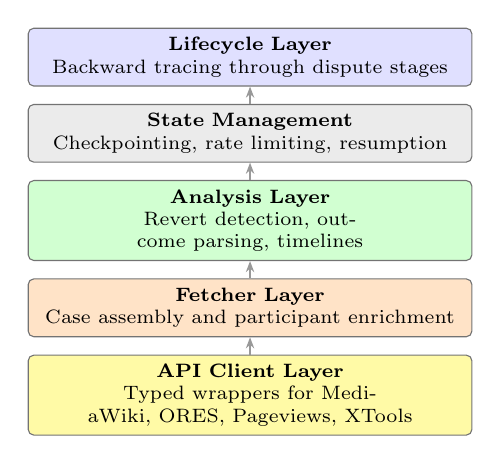
\begin{tikzpicture}[
  layer/.style={rectangle, draw=black!55, fill=#1,
                text width=5.4cm, align=center,
                minimum height=0.68cm, font=\scriptsize,
                rounded corners=2pt},
  fwd/.style={-{Stealth[length=4pt]}, draw=black!40, thick}
]
  \node[layer=blue!12]   (l5) {\textbf{Lifecycle Layer}\\Backward tracing through dispute stages};
  \node[layer=stagegray, below=0.22cm of l5] (l4) {\textbf{State Management}\\Checkpointing, rate limiting, resumption};
  \node[layer=green!18,  below=0.22cm of l4] (l3) {\textbf{Analysis Layer}\\Revert detection, outcome parsing, timelines};
  \node[layer=orange!22, below=0.22cm of l3] (l2) {\textbf{Fetcher Layer}\\Case assembly and participant enrichment};
  \node[layer=yellow!35, below=0.22cm of l2] (l1) {\textbf{API Client Layer}\\Typed wrappers for MediaWiki, ORES, Pageviews, XTools};
  \draw[fwd] (l1.north) -- (l2.south);
  \draw[fwd] (l2.north) -- (l3.south);
  \draw[fwd] (l3.north) -- (l4.south);
  \draw[fwd] (l4.north) -- (l5.south);
\end{tikzpicture}
\caption{Five-layer pipeline architecture. Each layer consumes outputs from
  the layer below. All source code is publicly available at~\cite{b_repo}.}
\label{fig:pipeline}
\end{figure}

\noindent\textbf{API Client Layer.}
Thin, typed wrappers over each external service expose methods covering
revisions, user info, block histories, abuse filter logs, page assessments,
protection logs, and log events.

\noindent\textbf{Fetcher Layer.}
High-level orchestration coordinates API calls to assemble a complete case
record: all five ArbCom subpages, enriched participant profiles with block
histories, article quality assessments and revision histories, and
cross-references to ANI and DRN archives.

\noindent\textbf{Analysis Layer.}
Post-collection analytics compute revert ratios, flag bilateral edit wars,
and extract structured sanctions and findings from ArbCom wikitext.

\noindent\textbf{State Management Layer.}
Each case transitions through states \textit{pending} $\rightarrow$
\textit{in\_progress} $\rightarrow$ \textit{completed} / \textit{failed}.
State is persisted every ten items and survives interruption. The
\texttt{make pull} command resumes from the last checkpoint automatically.

\noindent\textbf{Lifecycle Layer.}
For each ArbCom case, this layer traces the dispute backward through earlier
intervention stages, collecting talk page revisions, ANI archive sections
mentioning case participants, and DRN archive sections.

\subsection{Schema and Key Fields}

Each case produces one JSON document with sections for pages (wikitext +
revisions), enriched participant profiles, block histories, article quality
and protection data, ANI/DRN cross-references, and structured outcome
(sanctions, findings). Table~\ref{tab:keyfields} lists the fields most
relevant to the process model and downstream predictions.

\begin{table}[tb]
\caption{Key Schema Fields for Downstream Analysis}
\label{tab:keyfields}
\begin{tabularx}{\columnwidth}{@{}l X@{}}
\toprule
\textbf{Field} & \textbf{Research Use} \\
\midrule
\texttt{revisions[].tags}            & Revert detection without comment parsing \\
\texttt{participants[].edit\_count}   & Editor experience proxy \\
\texttt{participants[].is\_admin}     & Admin involvement in dispute \\
\texttt{part\_blocks[].reason}        & Policy violations tied to dispute \\
\texttt{abuse\_hits.by\_result}        & Disallowed actions and warnings \\
\texttt{articles[].quality\_class}    & Article salience (FA $>$ GA $>$ B \ldots) \\
\texttt{articles[].protection\_count} & Edit war severity proxy \\
\texttt{outcome.sanctions}           & Recipient and type of each sanction \\
\bottomrule
\end{tabularx}
\end{table}

\subsection{Reproducibility and Code Availability}

All source code, configuration files, and collected artifacts are publicly
available in a single GitHub repository~\cite{b_repo}. The repository is
structured so that any researcher can clone it, inspect every step of the
pipeline, and reproduce or extend the data collection. A \texttt{Makefile}
provides entry points for the full pull (\texttt{make pull}), analysis, and
dashboard launch. The interactive dashboard~\cite{b_dashboard} and its
BPMN diagram files are also included, enabling reviewers to explore the
process models without running any code.

% -----------------------------------------------------------------------
\section{Analysis}
% -----------------------------------------------------------------------

\subsection{Edit War Detection}

For each article in a case, we compute the \emph{revert ratio}:
\begin{equation}
r = \frac{|\{e \in E : \text{isRevert}(e)\}|}{|E|}
\end{equation}
where $E$ is the set of revisions and $\text{isRevert}(e)$ is true when
revision $e$ carries a recognized revert tag (\texttt{mw-revert},
\texttt{mw-reverted}) or when the edit comment matches a set of revert
keywords. Articles with $r > 0.10$ are flagged as contested; those where the
same two editors account for more than 60\% of mutual reverts are treated as
active bilateral edit wars.

Additionally, we apply the M-index from Yasseri et al.~\cite{b_yasseri2012} to
quantify the intensity of mutually reverting editor pairs:
\begin{equation}
M = \sum_{i < j} \min(r_{ij}, r_{ji})
\end{equation}
where $r_{ij}$ is the number of times editor $i$ reverted editor $j$.

\subsection{Escalation Lifecycle Reconstruction}

For each case we reconstruct the temporal sequence of dispute events across
venues using a \texttt{DisputeTimeline} data model. Each
\texttt{TimelineEntry} records a venue, timestamp, participant
set, and a reference to the raw revision or mention that produced it. The resulting
timeline enables measurement of:

\begin{itemize}
    \item \emph{Time-to-escalation}: days between first talk page post and
          first DRN/ANI filing.
    \item \emph{Venue overlap}: fraction of cases with detectable presence at
          three or more stages.
    \item \emph{Participant persistence}: fraction of disputants who appear
          at every stage of their case.
\end{itemize}

\subsection{Editor Co-occurrence Networks}

We model each resolved dispute as a bipartite graph $G = (U, V, E)$ where $U$
is the set of editors, $V$ is the set of dispute venues, and an edge
$(u, v) \in E$ indicates that editor $u$ was active at venue $v$. Projecting
onto $U$ yields an editor co-occurrence network: two editors are connected if
they appeared together at the same dispute venue. Repeated co-occurrence across
multiple cases forms the basis for identifying \emph{chronic conflictors} and
possible organized disruption.

% -----------------------------------------------------------------------
\section{Preliminary Results}
% -----------------------------------------------------------------------

\subsection{Sample Case Collection}

We collected complete lifecycle data for five high-profile ArbCom cases:
\textit{Climate change}, \textit{Gamergate}, \textit{Eastern Europe},
\textit{Scientology}, and \textit{Muhammad images}. These cases were selected
to span a range of dispute types (scientific consensus, harassment,
geopolitics, religion) and temporal periods (2004--2015).

For each case, the pipeline successfully retrieved all five ArbCom subpages,
enriched participant profiles, and linked corresponding ANI and DRN archive
sections. Total collection time per case ranged from 8--22 minutes at
authenticated API rate limits.

\subsection{Revert Patterns}

Across the five sample cases, article revert ratios ranged from 0.04 to
0.41. The \textit{Climate change} case articles exhibited a mean revert ratio
of 0.18; the \textit{Gamergate} case articles reached 0.35 on the core
article during the peak dispute window. Bilateral mutual reversion was
concentrated in two-editor pairs in four of the five cases, consistent with
the findings of Kittur et al.~\cite{b_kittur2007}.

\subsection{Participant Persistence Across Venues}

In all five cases, at least 60\% of editors named in the ArbCom evidence
subpage also appeared in ANI archive sections for the same dispute period. In
three cases, at least one participant had a prior ArbCom appearance under a
different case name, suggesting that a subset of editors are chronic
participants in formal dispute resolution.

\subsection{Outcome Parsing}

The outcome-parsing module successfully
extracted structured sanction records from ArbCom wikitext for all five cases. Sanctions included
topic bans (most common), supervised editing requirements, and one site ban.
In all cases, sanctioned participants had higher abuse filter hit counts than
unsanctioned participants (mean 4.2 vs.\ 0.8 hits per participant), providing
initial evidence for the feasibility of sanction prediction.

\subsection{Full Pull Progress}

As of the time of writing, the pipeline has completed collection for 80 of the
approximately 170 ArbCom cases in the master list, yielding approximately
115~MB of structured JSON data. The remaining cases are queued and will be
collected via the resumable pull system.

% -----------------------------------------------------------------------
\section{Discussion}
% -----------------------------------------------------------------------

\subsection{Editor Recurrence Across Venues}

The most consistent finding across our sample is that the same editors recur
across multiple dispute venues and across multiple cases over time. This supports
our central hypothesis: editor co-occurrence combined with temporal proximity
is the strongest linking signal for mapping dispute lifecycles. The implication
for platform governance is significant: a small number of chronic conflictors
may consume a disproportionate share of dispute resolution resources, motivating
early-identification tools that could allow preemptive intervention.

\subsection{Limitations}

Several limitations constrain the current analysis. First, the full pull is
not yet complete; findings may shift as later-era cases are incorporated.
Second, ArbCom cases are a selected sample of disputes: only those
irresolvable at lower stages reach arbitration, inducing survivor bias. Third,
our current escalation predictor is trained only on cases that escalated,
since DRN and 3O data collection is ongoing. Fourth, ORES enrichment has not
yet been integrated into the main pull, leaving ML-based revision quality
signals absent from the preliminary analysis.

\subsection{Ethical Considerations}

All data collection uses the public MediaWiki API under the Wikimedia
Foundation's terms of service. Editor usernames are present in the raw data
because they are already public on Wikipedia. Aggregated analysis and any
public dataset release will follow responsible disclosure practices consistent
with prior Wikipedia research~\cite{b_halfaker2013}.

% -----------------------------------------------------------------------
\section{Future Work}
% -----------------------------------------------------------------------

Immediate next steps for data collection are: (1)~complete the full
arbitration pull for all 170 cases; (2)~run an ORES enrichment pass over all
collected revision IDs to add damage and good-faith probabilities;
(3)~collect Pageviews data to test the hypothesis that high-traffic articles
attract more intense edit warring; and (4)~collect DRN cases to expand the
pre-ArbCom portion of the lifecycle.

\subsection{Escalation Prediction}

We plan to formulate escalation prediction as a binary classification task:
given talk page and ANI features for a dispute, predict whether the case will
reach ArbCom. Feature candidates include revert ratio, number of distinct
editors, presence of an administrator among participants, article quality
class, ORES damaging score distribution, and time since the dispute began.
We intend to evaluate logistic regression, gradient boosting, and a simple
transformer-based classifier over the talk page text.

\subsection{Sanction Outcome Classification}

A secondary modeling task will predict outcome severity for individual
participants given their behavioral signals: edit count, block history, abuse
filter hits, revert ratio contribution, and network centrality in the
co-occurrence graph. Outcome severity is defined across four levels: no
sanction, warning, topic ban, and site ban or indefinite block.

\subsection{Additional Planned Contributions}

Longer-term goals include a graph neural network over the editor co-occurrence
graph for chronic-conflicitor identification, a sequence-to-outcome model over
revision histories for sanction prediction, and an interactive visualization
dashboard of dispute lifecycle maps for the Lexipedia platform.

% -----------------------------------------------------------------------
\section{Conclusion}
% -----------------------------------------------------------------------

We presented a multi-stage framework for collecting and analyzing Wikipedia
dispute resolution data across all five intervention stages. Our pipeline
integrates four Wikimedia APIs into a unified, resumable collection system
that produces richly linked case records connecting participants, revisions,
articles, and outcomes. Preliminary analysis of five high-profile cases
demonstrates the feasibility of lifecycle reconstruction and surfaces systematic
patterns (bilateral revert concentration, editor persistence across stages,
and abuse filter hits as a sanction predictor) that motivate future modeling
work. The full dataset, once collected and released, will constitute the most
comprehensive longitudinal record of Wikipedia dispute escalation available to
researchers.

% -----------------------------------------------------------------------
\section*{Acknowledgment}
% -----------------------------------------------------------------------

The authors thank Professor Alvarado for guidance and feedback throughout the
project, and Anson and Lane at Lexipedia for domain expertise and access to
institutional knowledge of Wikipedia governance. This project was conducted
under the UVA MSDS Capstone program (DS~6015) in collaboration with Lexipedia
and the Wikimedia Foundation.

% -----------------------------------------------------------------------
\begin{thebibliography}{00}

\bibitem{b_wikistats}
Wikimedia Foundation, ``Wikipedia: Size comparisons,'' 2024.
[Online]. Available: \url{https://en.wikipedia.org/wiki/Wikipedia:Size_comparisons}

\bibitem{b_wp_disputes}
Wikipedia Contributors, ``Wikipedia: Dispute resolution,'' 2024.
[Online]. Available: \url{https://en.wikipedia.org/wiki/Wikipedia:Dispute_resolution}

\bibitem{b_wp_lifecycle}
Wikipedia Contributors, ``Wikipedia: Dispute resolution lifecycle,'' 2024.
[Online]. Available: \url{https://en.wikipedia.org/wiki/Wikipedia:Dispute_resolution}

\bibitem{b_wp_drn}
Wikipedia Contributors, ``Wikipedia: Dispute Resolution Noticeboard,'' 2024.
[Online]. Available: \url{https://en.wikipedia.org/wiki/Wikipedia:Dispute_resolution_noticeboard}

\bibitem{b_kittur2007}
A. Kittur, B. Suh, B. A. Pendleton, and E. H. Chi,
``He says, she says: Conflict and coordination in Wikipedia,''
in \textit{Proc. CHI 2007}, San Jose, CA, 2007, pp. 453--462.
DOI: \texttt{10.1145/1240624.1240698}

\bibitem{b_kittur2010}
A. Kittur and R. E. Kraut,
``Beyond Wikipedia: Coordination and conflict in online production groups,''
in \textit{Proc. CSCW 2010}, Savannah, GA, 2010, pp. 215--224.
DOI: \texttt{10.1145/1718918.1718963}

\bibitem{b_yasseri2012}
T. Yasseri, R. Sumi, A. Rung, A. Kornai, and J. Kert\'esz,
``Dynamics of conflicts in Wikipedia,''
\textit{PLoS ONE}, vol.~7, no.~6, e38869, 2012.
DOI: \texttt{10.1371/journal.pone.0038869}

\bibitem{b_halfaker2013}
A. Halfaker, R. S. Geiger, J. T. Morgan, and J. Riedl,
``The rise and decline of an open collaboration system: How Wikipedia's
reaction to popularity is causing its decline,''
\textit{American Behavioral Scientist}, vol.~57, no.~5, pp. 664--688, 2013.
DOI: \texttt{10.1177/0002764212469365}

\bibitem{b_geiger2010}
R. S. Geiger and D. Ribes,
``The work of sustaining order in Wikipedia: The banning of a vandal,''
in \textit{Proc. CSCW 2010}, Savannah, GA, 2010, pp. 117--126.
DOI: \texttt{10.1145/1718918.1718941}

\bibitem{b_taraborelli2010}
D. Taraborelli and G. L. Ciampaglia,
``Beyond notability: Collective deliberation on content inclusion in Wikipedia,''
in \textit{Proc. WikiSym 2010}, Gdansk, Poland, 2010.

\bibitem{b_kumar2014}
S. Kumar, F. Spezzano, V. S. Subrahmanian, and C. Faloutsos,
``Edge weight prediction in weighted signed networks,''
in \textit{Proc. IEEE ICDM 2014}, Shenzhen, China, 2014, pp. 221--230.
DOI: \texttt{10.1109/ICDM.2014.87}

\bibitem{b_welser2011}
H. T. Welser, D. Cosley, G. Kossinets, A. Lin, F. Dokshin, G. Gay, and M. Smith,
``Finding social roles in Wikipedia,''
\textit{American Behavioral Scientist}, vol.~55, no.~10, pp. 1358--1381, 2011.
DOI: \texttt{10.1177/0002764211414601}

\bibitem{b_zhang2018}
J. Zhang, J. Chang, C. Danescu-Niculescu-Mizil, L. Dixon, Y. Hua,
D. Taraborelli, and N. Thain,
``Conversations gone awry: Detecting early signs of conversational failure,''
in \textit{Proc. ACL 2018}, Melbourne, Australia, 2018, pp. 1350--1361.
DOI: \texttt{10.18653/v1/P18-1125}

\bibitem{b_cheng2015}
J. Cheng, C. Danescu-Niculescu-Mizil, and J. Leskovec,
``Antisocial behavior in online discussion communities,''
in \textit{Proc. ICWSM 2015}, Oxford, UK, 2015.

\bibitem{b_halfaker2011}
A. Halfaker, A. Kittur, and J. Riedl,
``Don't bite the newbies: How reverts affect the quantity and
quality of Wikipedia work,''
in \textit{Proc. WikiSym 2011}, Mountain View, CA, 2011, pp. 163--172.
DOI: \texttt{10.1145/2038558.2038585}

\bibitem{b_repo}
L. Cocks, K. Kelleher, and R. Healy,
``Wikipedia Dispute Models,'' GitHub, 2026.
[Online]. Available: \ghrepo

\bibitem{b_dashboard}
K. Kelleher, L. Cocks, and R. Healy,
``Arbitration Dashboard,'' GitHub, 2026.
[Online]. Available:
\href{https://github.com/rah-ds/Wikipedia_Dispute_Models/tree/main/dashboard}{\texttt{rah-ds/Wikipedia\_Dispute\_Models/dashboard}}

\bibitem{b_bpmn}
Object Management Group,
``Business Process Model and Notation (BPMN), Version 2.0,''
OMG Std., 2011. [Online]. Available: \url{https://www.omg.org/spec/BPMN/2.0}

\bibitem{b_bpmnjs}
Camunda Services GmbH,
``bpmn-js: BPMN 2.0 rendering toolkit for the web,'' 2024.
[Online]. Available: \url{https://github.com/bpmn-io/bpmn-js}

\bibitem{b_vander2012}
W. van der Aalst,
\textit{Process Mining: Discovery, Conformance and Enhancement of
Business Processes}.
Berlin: Springer, 2011.
DOI: \texttt{10.1007/978-3-642-19345-3}

\end{thebibliography}

\end{document}
